\documentclass[a4paper]{report}
\usepackage{float}
\usepackage[utf8]{inputenc}
\usepackage[italian]{babel}
\usepackage{amsmath}
\usepackage{amssymb}
\usepackage{graphicx}
\graphicspath{ {./graph/} }
\usepackage{lmodern}
\usepackage{kpfonts}
\usepackage{titlesec}
\usepackage{listings}
\usepackage{color}
\usepackage{fontspec}
\usepackage{multirow}
\usepackage{float}
\usepackage{array}
\usepackage{afterpage}

\usepackage[font={small}, labelfont={bf}, format=hang, skip=8pt]{caption}



\setmainfont{Helvetica} % Set the main font to Helvetica
\setmonofont{Noto Sans Mono} % Set the monofont to Andale Mono

% Imposta lo spacing tra il titolo del paragrafo e il testo successivo
\usepackage[left=3.6cm,right=3.6cm,top=2.5cm,bottom=2.25cm]{geometry}

\definecolor{grigio}{rgb}{0.95,0.95,0.95}
\definecolor{mygrey}{rgb}{0.8,0.8,0.8}
\definecolor{mygreen}{rgb}{0.2,0.4,0.2}

\lstset{
    firstnumber=1,                % start line enumeration with line 1000
    language=Verilog,
    numbers=left,
    stepnumber=1,
    numbersep=4pt,
    numberstyle=\tiny\color{mygrey}, % the style that is used for the line-numbers
    backgroundcolor=\color{grigio},
    showspaces=false,
    showstringspaces=false,
    showtabs=false,
    tabsize=3,
    captionpos=b,
    breaklines=true,
    breakatwhitespace=true,
    escapeinside={\%*}{*)},
    basicstyle=\ttfamily\fontsize{8pt}{10pt}\selectfont, % Set the basic code style to a smaller font
    keywordstyle=\bfseries,
    commentstyle=\color{mygreen}}

\titleformat{\chapter}[display]
{\normalfont\huge\bfseries\fontsize{14pt}{10pt}\selectfont}{\chaptertitlename\ \thechapter}{18pt}{\Huge}

\author{Tommi Bimbato VR500751, Antonio Iovine VR504083}
\title{Elaborato Sis e Verilog \\ \normalsize Corso di Architettura degli Elaboratori A.A. 2023/2024 \\ Prof.\ Franco Fummi, Prof.\ Michele Lora}


\begin{document}

\begin{titlepage}
    \maketitle
\end{titlepage}

% Applica il nuovo stile di intestazione a tutte le pagine tranne la prima
\thispagestyle{empty} % Rimuove l'intestazione dalla pagina del titolo

\tableofcontents % Aggiunge una tabella dei contenuti

\begin{abstract}
Questa relazione presenta una descrizione dettagliata del progetto sviluppato in SIS e Verilog per il gioco della "Morra Cinese". Vengono illustrati i concetti principali, le scelte progettuali e i risultati ottenuti.
In allegato alla presente relazione sono presenti i codici SIS e Verilog inerenti al progetto.
L'elaborato è stato eseguito da Tommi Bimbato e Antonio Iovine durante il primo semestre del corso di Architettura degli Elaboratori tenuto dai professori Franco Fummi e Michele Lora nell'A.A. 2023/2024.

\end{abstract}

\chapter{Introduzione}
\section{Approccio progettuale}
L'elaborato è stato inizialmente analizzato e sviluppato a partire da una risoluzione algorithmica delle specifiche e dei requisiti di output \textit{(Linguaggio C)}.
Successivamente, è stato elaborato un possibile schema di funzionamento del sistema (FSMD), sono state individuate le componenti più affini al calcolo combinatorio e la loro controparte nell'esecuzione in FSM (vedere sezione \ref{sec:approfondimento}).\@
Una volta suddivise le funzioni tra Datapath e controllore (FSM), si è descritto in codice verilog il comportamento generale della macchina.
Si è passati contemporaneamente alla progettazione a \textit{gate level} dei componenti del datapath confrontando il comportamento del modello in Verilog e i singoli blocchi che compongono il Datapath.\@

\section{Analisi delle specifiche}
\subsection{Specifiche di input e output}
Le specifiche impongono questa configurazione di input e output principali:
\begin{itemize}
    \item \textbf{Input}
    \begin{itemize}
        \item \texttt{PRIMO}: segnale a 2 bit che rappresenta la scelta del giocatore 1 (tabella \ref{tab:mosse})
        \item \texttt{SECONDO}: segnale a 2 bit che rappresenta la scelta del giocatore 2 (tabella \ref{tab:mosse})
        \item \texttt{INIZIA}: segnale a 1 bit che funge da input per il reset e l'inizio della partita
    \end{itemize}
    \item \textbf{Output}
    \begin{itemize}
        \item \texttt{MANCHE}: segnale a 2 bit che rappresenta il vincitore della manche (tabella \ref{tab:manche})
        \item \texttt{PARTITA}: segnale a 2 bit che rappresenta la fine della manche (tabella \ref{tab:partita})
    \end{itemize}
\end{itemize}

\begin{figure}[h]
  \centering
  \begin{minipage}[t]{0.45\linewidth}
    \centering
    \renewcommand{\arraystretch}{1.4}
    \begin{tabular}{|c|c|}
        \hline
        \textbf{PRIMO/SECONDO} & \textbf{Codifica in bit} \\
        \hline
        Sasso & 01 \\
        \hline
        Carta & 10 \\
        \hline
        Forbice & 11 \\
        \hline
        Mossa non valida & 00 \\
        \hline
    \end{tabular}
    \captionof{table}{\small Codifica di PRIMO e SECONDO}
    \label{tab:mosse}
  \end{minipage}
  \begin{minipage}[t]{0.45\linewidth}
    \centering
    \renewcommand{\arraystretch}{1.4}
    \begin{tabular}{|c|c|}
        \hline
        \textbf{MANCHE} & \textbf{Codifica in bit} \\
        \hline
        Vittoria G1 & 01 \\
        \hline
        Vittoria G2 & 10 \\
        \hline
        Pareggio & 11 \\
        \hline
        Manche annullata & 00 \\
        \hline
    \end{tabular}
    \captionof{table}{\small Codifica di MANCHE}
    \label{tab:manche}
  \end{minipage}

  \vspace{10pt}

  \begin{minipage}[t]{0.5\linewidth}
    \centering
    \renewcommand{\arraystretch}{1.4}
    \begin{tabular}{|c|c|}
      \hline
      \textbf{PARTITA} & \textbf{Codifica} \\
      \hline
      Vince PRIMO & 01 \\
      \hline
      Vince SECONDO & 10 \\
      \hline
      Pareggio & 11 \\
      \hline
      Partita in corso & 00 \\
      \hline
    \end{tabular}
    \captionof{table}{\small Codifica di PARTITA}
    \label{tab:partita}
  \end{minipage}
\end{figure}


\subsection{Specifiche di funzionamento e regole del gioco}
\subsubsection*{Dinamica di gioco}

Quando il segnale \texttt{INIZIA} viene impostato a 1, il sistema si resetta e si prepara per una nuova serie di manche.
Il numero massimo di manche che possono essere giocate in una partita è determinato dalla concatenazione dei bit di \texttt{PRIMO} e \texttt{SECONDO}, a cui viene aggiunto il valore minimo di manche giocabili (4).
La partita si divide in manche, durante le quali ciascuno dei due giocatori sceglie una tra tre mosse: \texttt{SASSO}, \texttt{CARTA} e \texttt{FORBICE}.
Questa scelta avviene simultaneamente per entrambi i giocatori, e viene rappresentata attraverso gli input \texttt{PRIMO} e \texttt{SECONDO}.
Una volta che entrambi i giocatori hanno effettuato la loro mossa, il sistema elabora le scelte e determina il vincitore della manche e lo descrive tramite l'output \texttt{MANCHE}.\@
\\

\subsubsection*{Regola della mossa ripetuta da un uscente vinciore}
In addizione alla regola standard per la definizione del vincitore della manche è stata aggiunta nelle specifiche una regola che si attiva alla ripetizione della mossa da parte del vincitore uscente da una manche.
Se un giocatore vince una manche, nella successiva non potrà riutilizzare la stessa mossa, in caso contrario la manche sarà nulla fintanto che il giocatore non cambierà mossa.

\subsubsection*{Vincitore in caso di raggiungimento delle partite massime}
Il vincitore della partita è il primo giocatore che raggiunge un vantaggio di due manche sull'altro giocatore.
In termini progettuali questa affermazione \textit{potrebbe} nascondere un ambiguità: il sistema è stato quindi progettato affinchè in caso di raggiungimento del numero di manche massime con un giocatore in vantaggio di una sola manche la vittoria sarà assegnata anche se non è soddisfatta la specifica $ Vantaggio = 2 $.

\chapter{FSDM (Finish State Machine with Datapath)}
Il sistema di controllo tramite FSM gestisce il controllo a partire dall'elaborazione del datapath delle singole manche.
Gli ingressi del sistema sono direttamente collegati al datapath che calcola, per ogni manche, il vincitore. Questo dato (sotto forma di segnale a 2 bit), vine passato alla FSM che si occupa di gestire il flusso dei segnali di output.
Il Datapath passa inoltre all'FSM 2 segnali di controllo che si attivano al superamento delle 4 manche minime giocate e al raggiungimento del numero massimo di manche giocabili\footnote{Nello specifico \texttt{CMIN} sale ad 1 quando sono state giocate 4 manche e \texttt{CMAX} sale ad 1 quando sono state giocate le manche massime.}.

    \begin{figure}[h]
        \centering
        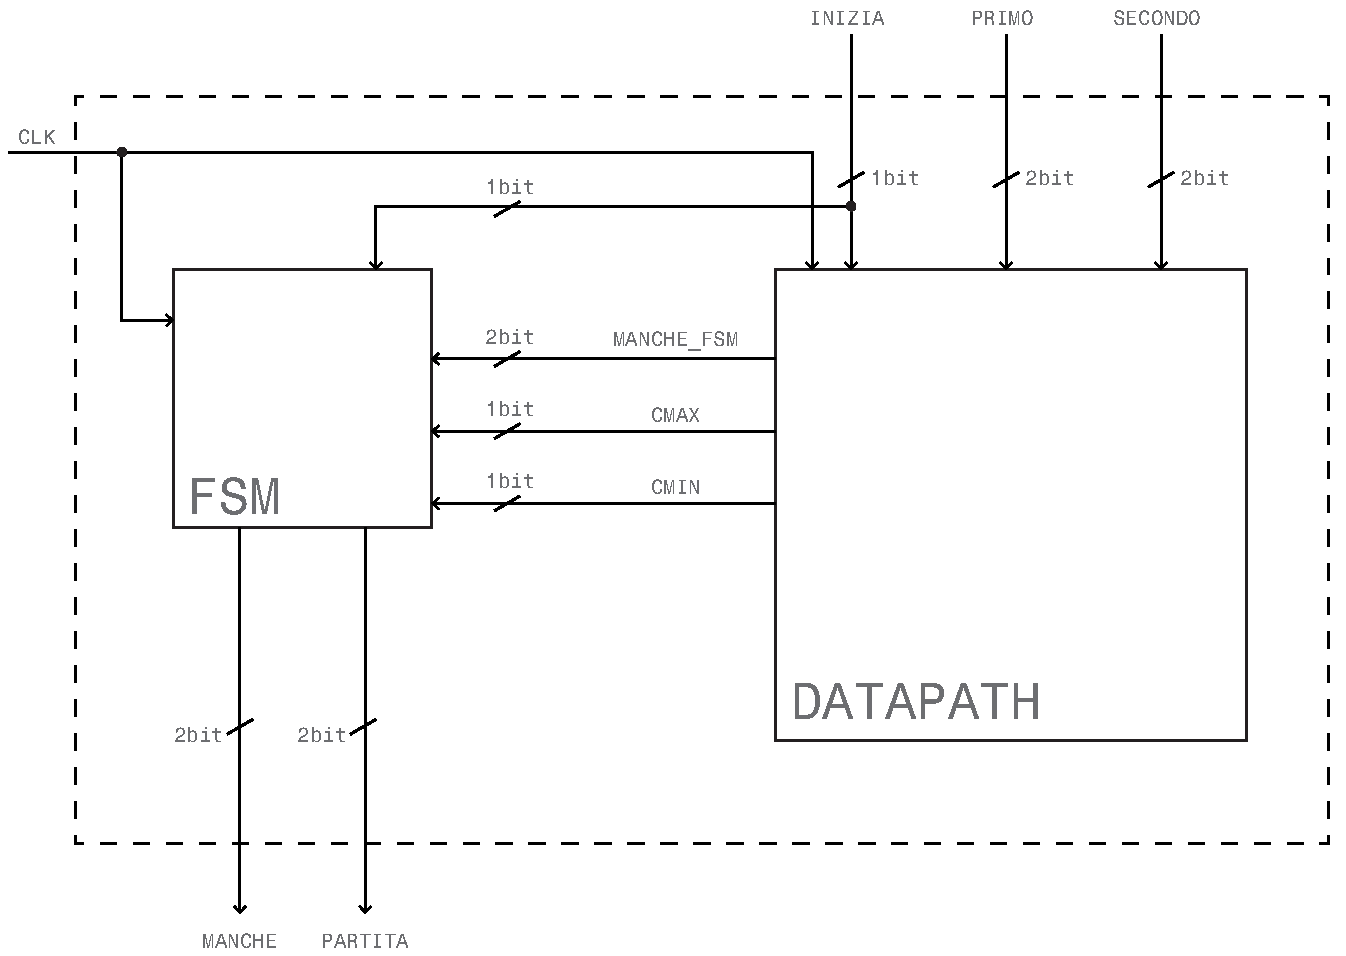
\includegraphics[width=\textwidth]{FSMD_generale.pdf}
        \caption[FSMD]{Schema di funzionamento generale dell'FSMD}
        \label{img:FSMD}
    \end{figure}


\section{Datapath}

Il Datapath è il componente che si occupa di elaborare le scelte dei giocatori e determinare il vincitore della manche.
Nonostante abbiano approcci differenti nella descrizione hardware, sia utilizzando SIS a livello di gate che scrivendo codice Verilog in uno stile behavioural, il datapath presenta un comportamento coerente e equivalente in entrambe le rappresentazioni.

\subsection{Funzioni Principali del Datapath}

\subsubsection{Reset e Inizializzazione dei Registri}
La funzione di reset e inizializzazione dei registri permette al sistema di tornare ad una configurazione coerente e prevedibile all'inizio di una nuova partita.
Il segnale \texttt{INIZIA} è collegato direttamente al Datapath e viene utilizzato per la sopracitata funzione.

\subsubsection{Settaggio del Numero di Manche Massime}
Il Datapath è incaricato di impostare il numero massimo di manche per la partita.
Questo valore è basato sulla concatenazione dei bit rappresentanti le scelte dei giocatori (\texttt{PRIMO} e \texttt{SECONDO}) e un valore minimo di manche giocabili (4).
In concreto questa funzione viene eseguita registrando in un registro a 5 bit il valore di \texttt{PRIMO} e \texttt{SECONDO} concatenati e sommando 4.

\subsubsection{Calcolo combinatorio del vincitore della \textit{manche} e applicazione delle regole interne}
Una delle funzioni più cruciali del Datapath è determinare la mossa vincente tra le due prese in input (\texttt{PRIMO} e \texttt{SECONDO}).
Durante la progettazione a gate level (ambiente SIS), per garantire la correttezza e comprensibilità del percorso dei segnali, abbiamo adottato una strategia di codifica degli input \texttt{PRIMO} e \texttt{SECONDO}.
Questi input, rappresentanti le mosse dei giocatori, sono stati convertiti in segnali a 3 bit ciascuno, dove ogni bit corrisponde ad una mossa\footnote{In ambiente verilog questa codifica non è stata necessaria vista la più alta astrazione dell'ambiente stesso e la possibilità di confrontare le mosse direttamente a 2 bit con un costrutto \textit{case}}.
La codifica inziale, (tabella \ref{tab:mosse}), consente una rappresentazione chiara e compatta delle mosse ma difficilmente confrontabile direttamente a gate level. Per fare questo è stato modellato il componente \texttt{"2b\_to\_3b.blif"} (vedere sezione \ref{subsec:component}) che converte la codifica binaria di PRIMO e SECONDO in una codifica a 3 bit.
Il Datapath gestisce anche le regole che coinvolgono la ripetizione della mossa da parte del vincitore uscente attraverso la memorizzazione in un registro dell'ultimo vincitore e della mossa utilizzata per la vittoria, confrontandolo quando necessario con la mossa giocata nella manche corrente. 

\subsubsection{Conteggio delle Manche Giocate e Invio di Segnali di Controllo all'FSM}
Il Datapath tiene traccia del numero di manche giocate e invia segnali di controllo specifici all'FSM.
Questi segnali contribuiscono al corretto flusso di gioco e determinano il passaggio agli stati successivi dell'FSM, in particolare dal Datapath escono il segnale di controllo \texttt{CMIN} e \texttt{CMAX}.
All'interno del datapath è presente un contatore a 5 bit che confronta la sua configurazione con il registro che contiene il numero massimo di manche impostato all'inizio della partita.
Il contatore di manche giocate reagisce anche alla possibilità di manche annullata: in questo caso il componente viene bypassato e il conteggio rimane statico fino alla sucessiva manche valida.

\section{Finish State Machine}

L'FSM è il componente che si occupa di gestire il flusso dei segnali di output e di controllo, è stata ideata ad 8 stati e secondo il modello della macchina di Mealy.
Il controllore FSM procede a decretare il vincitore se le condizioni per farlo sono soddisfatte tenendo conto dei vantaggi che accumulano i rispettivi giocatori.
Lo stato iniziale dell'FSM è \texttt{S0} (tabella \ref{tab:codifica_stati}), da questo varia in base all'esito del segnale che determina il vincitore da ogni manche in arrivo dal Datapath.
Quando sussistono le condizioni per la vittoria della partita o terminano le manche giocabili il controllore decreta il vincitore tramite L'output \texttt{PARTITA} e torna allo stato iniziale qualora l'input principale \texttt{INIZIA} salga ad 1 stimolando il reset.
\\
Il \textit{controllore FSM} prende in input 4 segnali:
\begin{itemize}
    \item \texttt{MANCHE\_FSM}: segnale a 2 bit che rappresenta il vincitore della manche da passare alla FSM.
    \item \texttt{CMIN}: segnale a 1 bit che si attiva al raggiungimento delle 4 manche minime.
    \item \texttt{CMAX}: segnale a 1 bit che si attiva al raggiungimento delle manche massime.
    \item \texttt{INIZIA}: segnale a 1 bit che funge da input per il reset e l'inizio della partita e che permette di riportare la FSM allo stato iniziale.
\end{itemize}

Ed emette in output i 2 segnali principali:
\begin{itemize}
    \item \texttt{MANCHE}: segnale a 2 bit che rappresenta il vincitore della manche.
    \item \texttt{PARTITA}: segnale a 2 bit che decreta il vincitore dell'intera partita.
\end{itemize}

\vspace*{10pt}
\begin{center}
    La codifica binaria degli stati è stata impostata secondo il seguente schema:
        \begin{table}[h]
            \centering
        \renewcommand{\arraystretch}{1.4}
        \ttfamily

        \begin{tabular}{|c|c|c|}
        \hline
        \textbf{Nome stato} & \textbf{Codifica} & \textbf{Descrizione} \\
        \hline
        S0 & 000 & INIT / Pareggio  \\
        \hline
        S1 & 001 & Vantaggio di PRIMO = 1 \\
        \hline
        S2 & 010 & Vantaggio di PRIMO = 2 \\
        \hline
        S3 & 011 & Vantaggio di PRIMO = 3 \\
        \hline
        S4 & 100 & Vantaggio di SECONDO = 1 \\
        \hline
        S5 & 101 & Vantaggio di SECONDO = 2 \\
        \hline
        S6 & 110 & Vantaggio di SECONDO = 3 \\
        \hline
        S7 & 111 & Partita conclusa \\
        \hline
        \end{tabular}
        \caption{Codifica degli stati dell'FSM}
        \label{tab:codifica_stati}
        \end{table}
\end{center}

La combinazione degli input secondari (MANCHE\_FSM, CMIN, CMAX), l'ingresso principale \texttt{INIZIA} e lo stato corrente dell'automa determinano lo stato prosimo ($\delta$) e gli output (secondo la funzione di output $\lambda$).
In uscita alla FSM ci sono le due uscite principali del sistema: \texttt{MANCHE} (2bit) e \texttt{PARTITA} (2bit).
I passaggi di stato e le uscite sono descritti in dettaglio nella tabella \ref{tab:mealy} e nel diagramma dei passaggi di stato (figura \ref{img:fsmtg}).


\begin{figure}[ht]
  \centering
  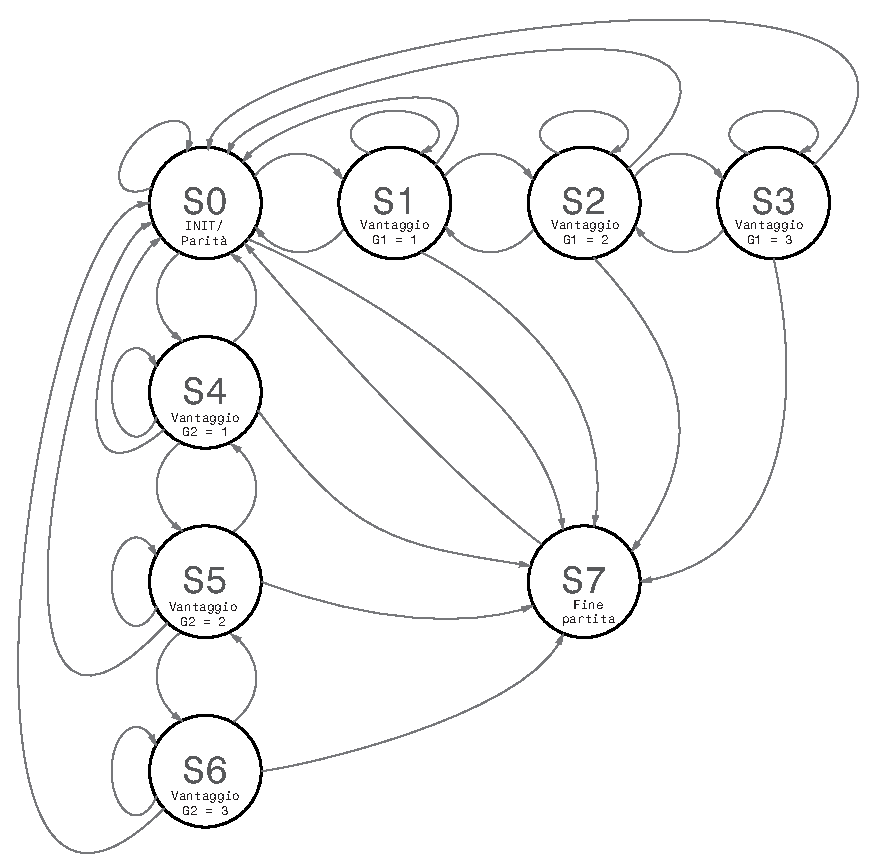
\includegraphics[width=\textwidth]{FSMTG.pdf}
  \caption{State Transition Graph}
  \label{img:fsmtg}
\end{figure}


\begin{center}
  \begin{table}[h]
      \centering
  \renewcommand{\arraystretch}{1.2}
  \footnotesize
  \ttfamily
  \begin{tabular}{|c|c|c|c|}
      \hline
      \textbf{Input} & \textbf{Stato Attuale} & \textbf{Stato Prossimo} & \textbf{Output}\\
      \hline
      \textbf{MANCHE\_FSM - CMIN - CMAX - INIZIA} &  &  & \textbf{MANCHE - PARTITA} \\ 
      \hline

      \ \  00 \ \ - \ \ - \ \ 0 & S0 & S0 & 00 \ \ 00 \\
      \cline{1-4} \ \ 
      11 \ \ 0 \ \ 0 \ \ 0 & S0 & S0 & 11 \ \ 00 \\
      \cline{1-4} \ \ 
      00 \ \ - \ \ - \ \ 0 & S1 & S1 & 00 \ \ 00 \\
      \cline{1-4} \ \ 
      11 \ \ 0 \ \ 0 \ \ 0 & S1 & S1 & 11 \ \ 00 \\
      \cline{1-4} \ \ 
      00 \ \ - \ \ - \ \ 0 & S2 & S2 & 00 \ \ 00 \\
      \cline{1-4} \ \ 
      11 \ \ 0 \ \ 0 \ \ 0 & S2 & S2 & 11 \ \ 00 \\
      \cline{1-4} \ \ 
      00 \ \ - \ \ - \ \ 0 & S3 & S3 & 00 \ \ 00 \\
      \cline{1-4} \ \ 
      11 \ \ 0 \ \ 0 \ \ 0 & S3 & S3 & 11 \ \ 00 \\
      \cline{1-4} \ \ 
      01 \ \ - \ \ 0 \ \ 0 & S0 & S1 & 01 \ \ 00 \\
      \cline{1-4} \ \ 
      01 \ \ 0 \ \ 0 \ \ 0 & S1 & S2 & 01 \ \ 00 \\
      \cline{1-4} \ \ 
      01 \ \ 0 \ \ 0 \ \ 0 & S2 & S3 & 01 \ \ 00 \\
      \cline{1-4} \ \ 
      10 \ \ 0 \ \ 0 \ \ 0 & S3 & S2 & 10 \ \ 00 \\
      \cline{1-4} \ \ 
      10 \ \ - \ \ 0 \ \ 0 & S2 & S1 & 10 \ \ 00 \\
      \cline{1-4} \ \ 
      10 \ \ - \ \ 0 \ \ 0 & S1 & S0 & 10 \ \ 00 \\
      \cline{1-4} \ \ 
      00 \ \ - \ \ - \ \ 0 & S4 & S4 & 00 \ \ 00 \\
      \cline{1-4} \ \ 
      11 \ \ 0 \ \ 0 \ \ 0 & S4 & S4 & 11 \ \ 00 \\
      \cline{1-4} \ \ 
      00 \ \ - \ \ - \ \ 0 & S5 & S5 & 00 \ \ 00 \\
      \cline{1-4} \ \ 
      11 \ \ 0 \ \ 0 \ \ 0 & S5 & S5 & 11 \ \ 00 \\
      \cline{1-4} \ \ 
      00 \ \ - \ \ - \ \ 0 & S6 & S6 & 00 \ \ 00 \\
      \cline{1-4} \ \ 
      11 \ \ 0 \ \ 0 \ \ 0 & S6 & S6 & 11 \ \ 00 \\
      \cline{1-4} \ \ 
      10 \ \ - \ \ 0 \ \ 0 & S0 & S4 & 10 \ \ 00 \\
      \cline{1-4} \ \ 
      10 \ \ 0 \ \ 0 \ \ 0 & S4 & S5 & 10 \ \ 00 \\
      \cline{1-4} \ \ 
      10 \ \ 0 \ \ 0 \ \ 0 & S5 & S6 & 10 \ \ 00 \\
      \cline{1-4} \ \ 
      01 \ \ 0 \ \ 0 \ \ 0 & S6 & S5 & 01 \ \ 00 \\
      \cline{1-4} \ \ 
      01 \ \ - \ \ 0 \ \ 0 & S5 & S4 & 01 \ \ 00 \\
      \cline{1-4} \ \ 
      01 \ \ - \ \ 0 \ \ 0 & S4 & S0 & 01 \ \ 00 \\
      \cline{1-4} \ \ 
      11 \ \ - \ \ 1 \ \ 0 & S0 & S7 & 11 \ \ 11 \\
      \cline{1-4} \ \ 
      01 \ \ - \ \ 1 \ \ 0 & S0 & S7 & 01 \ \ 01 \\
      \cline{1-4} \ \ 
      10 \ \ - \ \ 1 \ \ 0 & S0 & S7 & 10 \ \ 10 \\
      \cline{1-4} \ \ 
      11 \ \ - \ \ 1 \ \ 0 & S1 & S7 & 11 \ \ 01 \\
      \cline{1-4} \ \ 
      01 \ \ 1 \ \ - \ \ 0 & S1 & S7 & 01 \ \ 01 \\
      \cline{1-4} \ \ 
      10 \ \ - \ \ 1 \ \ 0 & S1 & S7 & 10 \ \ 11 \\
      \cline{1-4} \ \ 
      11 \ \ 1 \ \ - \ \ 0 & S2 & S7 & 11 \ \ 01 \\
      \cline{1-4} \ \ 
      01 \ \ 1 \ \ - \ \ 0 & S2 & S7 & 01 \ \ 01 \\
      \cline{1-4} \ \ 
      10 \ \ - \ \ 1 \ \ 0 & S2 & S7 & 10 \ \ 01 \\
      \cline{1-4} \ \ 
      11 \ \ 1 \ \ - \ \ 0 & S3 & S7 & 11 \ \ 01 \\
      \cline{1-4} \ \ 
      01 \ \ 1 \ \ - \ \ 0 & S3 & S7 & 01 \ \ 01 \\
      \cline{1-4} \ \ 
      10 \ \ 1 \ \ - \ \ 0 & S3 & S7 & 10 \ \ 01 \\
      \cline{1-4} \ \ 
      11 \ \ - \ \ 1 \ \ 0 & S4 & S7 & 11 \ \ 10 \\
      \cline{1-4} \ \ 
      01 \ \ - \ \ 1 \ \ 0 & S4 & S7 & 01 \ \ 11 \\
      \cline{1-4} \ \ 
      10 \ \ 1 \ \ - \ \ 0 & S4 & S7 & 10 \ \ 10 \\
      \cline{1-4} \ \ 
      11 \ \ 1 \ \ - \ \ 0 & S5 & S7 & 11 \ \ 10 \\
      \cline{1-4} \ \ 
      01 \ \ - \ \ 1 \ \ 0 & S5 & S7 & 01 \ \ 10 \\
      \cline{1-4} \ \ 
      10 \ \ 1 \ \ - \ \ 0 & S5 & S7 & 10 \ \ 10 \\
      \cline{1-4} \ \ 
      11 \ \ 1 \ \ - \ \ 0 & S6 & S7 & 11 \ \ 10 \\
      \cline{1-4} \ \ 
      01 \ \ 1 \ \ - \ \ 0 & S6 & S7 & 01 \ \ 10 \\
      \cline{1-4} \ \ 
      10 \ \ 1 \ \ - \ \ 0 & S6 & S7 & 10 \ \ 10 \\
      \cline{1-4} \ \ 
      -- \ \ - \ \ - \ \ 1 & S0 & S0 & 00 \ \ 00 \\
      \cline{1-4} \ \ 
      -- \ \ - \ \ - \ \ 1 & S1 & S0 & 00 \ \ 00 \\
      \cline{1-4} \ \ 
      -- \ \ - \ \ - \ \ 1 & S2 & S0 & 00 \ \ 00 \\
      \cline{1-4} \ \ 
      -- \ \ - \ \ - \ \ 1 & S3 & S0 & 00 \ \ 00 \\
      \cline{1-4} \ \ 
      -- \ \ - \ \ - \ \ 1 & S4 & S0 & 00 \ \ 00 \\
      \cline{1-4} \ \ 
      -- \ \ - \ \ - \ \ 1 & S5 & S0 & 00 \ \ 00 \\
      \cline{1-4} \ \ 
      -- \ \ - \ \ - \ \ 1 & S6 & S0 & 00 \ \ 00 \\
      \cline{1-4} \ \ 
      -- \ \ - \ \ - \ \ 1 & S7 & S0 & 00 \ \ 00 \\
      \cline{1-4} \ \ 
      -- \ \ - \ \ - \ \ 0 & S7 & S7 & 00 \ \ 00 \\
      \cline{1-4}
      \hline
      \end{tabular}
      \caption{Descrizione input e output dei passaggi di stato dell'FSM}
      \label{tab:mealy}
    \end{table}
\end{center}



\chapter{Verilog}
\section{Design.sv}
Contesualmente alla presente relazione è stato allegato il codice \texttt{design.sv} contenente la descrizione hardware del sistema in linguaggio Verilog.
Nella prima parte della descrizione hardware vengono dichiarate le porte di input e output del sistema e i registri necessari.
Oltre agli input e output principali definiti nelle specifiche, sono stati aggiunti dei registri per il controllo del numero di manche settate e giocate, la memorizzazione dell'ultima mossa vincente e i segnali di controllo scambiati tra il datapath e l'FSM.\@
Vengono inoltre specificati i parametri locali di tutti possibili stati della FSM.

\begin{lstlisting}
  module MorraCinese (
  // Inputs
  input [1:0] PRIMO,
  input [1:0] SECONDO,
  input INIZIA,
  input clk,
  // Outputs
  output reg [1:0] MANCHE = 2'b00,
  output reg [1:0] PARTITA = 2'b00
);

  reg [1:0] MOSSA_PRECEDENTE = 2'b00;
  reg [4:0] NUMERO_PARTITE = 5'b00000;
  reg [4:0] CONTATORE = 5'b00000;
  reg [1:0] MANCHE_REG = 2'b00;
  reg [2:0] STATO = 3'b000;
  reg [2:0] STATO_PROSSIMO;
  reg CMIN = 1'b0;
  reg CMAX = 1'b0;

  reg [1:0] MANCHE_FSM;
  integer i = 1; // Debug purpose

  localparam S0 = 3'b000,
              S1 = 3'b001,
              S2 = 3'b010,
              S3 = 3'b011,
              S4 = 3'b100,
              S5 = 3'b101,
              S6 = 3'b110,
              S7 = 3'b111;

\end{lstlisting}

\vspace{20pt}

Viene descritto un blocco sincorno che al variare del Clock aggiorna lo stato della FSM con lo stato prossimo calcolato nell'FSM.

\begin{lstlisting}[firstnumber=34]
  always @(posedge clk) begin : UPDATE_STATE
    STATO = STATO_PROSSIMO;
  end;

\end{lstlisting}


\vspace{20pt}

Ad ogni fronte di salita del segnale di clock (\texttt{posedge clk}) si procede con il reset iniziale in risposta al segnale \texttt{INIZIA}.
Durante il reset, vengono inizializzati i registri e i segnali di controllo del sistema e lo stato dell'FSM.
Successivamente, mediante una serie di condizioni e case statement si gestiscono le diverse combinazioni di mosse dei giocatori e vengono applicate le regole del gioco.
La variabile \texttt{MANCHE\_FSM} rappresenta lo stato della manche, mentre \texttt{MOSSA\_PRECEDENTE} memorizza la mossa vincente precedente.
Si procede con conteggio delle manche e la verifica del raggiungimento delle manche minime e massime e vengono eventualmente inviati alla FSM i segnali di controllo \texttt{CMIN} e \texttt{CMAX}.
La descrizione include anche ritardi (\texttt{\#1}), questa pausa è stata inserita dopo la sezione di reset iniziale quando il segnale INIZIA è attivo.
L'obiettivo è dare il tempo al sistema di completare l'operazione di reset prima di procedere con le operazioni successive.\footnote{Poiché la simulazione in Verilog è discreta e avviene a passi di tempo discreti (cicli di clock), è necessario introdurre un ritardo per garantire che il sistema si trovi in uno stato coerente prima di eseguire ulteriori operazioni.}



\begin{lstlisting}[firstnumber=38]
  always @(posedge clk) begin : DATAPATH
  if (INIZIA) begin
    MOSSA_PRECEDENTE  = 2'b00;
    PARTITA           = 2'b00;
    MANCHE_REG        = 2'b00;
    MANCHE_FSM        = 2'b00;
    MANCHE            = 2'b00;
    CMAX              = 1'b0;
    CMIN              = 1'b0;
    NUMERO_PARTITE    = {PRIMO, SECONDO} + 4;
    CONTATORE         = 5'b00000;  
    STATO             = 3'b000;
  end else begin
    // Datapath core logic
    if ({MOSSA_PRECEDENTE, MANCHE_REG} == {PRIMO, 2'b01} || {MOSSA_PRECEDENTE, MANCHE_REG} == {SECONDO, 2'b10}) begin
      MANCHE_FSM = 2'b00;
    end else begin
      case ({PRIMO, SECONDO}) 
        4'b0101, 4'b1010, 4'b1111: begin
          MANCHE_FSM = 2'b11;
          MOSSA_PRECEDENTE = 2'b00;
        end
        4'b0111, 4'b1001, 4'b1110, 4'b0100, 4'b1000, 4'b1100 : begin
          MANCHE_FSM = 2'b01;
          MOSSA_PRECEDENTE = {PRIMO};
        end
        4'b0110, 4'b1011, 4'b1101, 4'b0001, 4'b0010, 4'b0011: begin
          MANCHE_FSM = 2'b10;
          MOSSA_PRECEDENTE = {SECONDO};
        end
        4'b0000: begin
          MANCHE_FSM = 2'b00;
          MOSSA_PRECEDENTE = 2'b00;
        end
      endcase
      if (MANCHE_FSM != 2'b00) begin
        MANCHE_REG = MANCHE_FSM;
        CONTATORE = CONTATORE + 1;
      end
    end
            
    if (CONTATORE == 4)
      CMIN = 1'b1;
    if (CONTATORE == NUMERO_PARTITE) 
      CMAX = 1'b1;     
  end
  #10;
end

\end{lstlisting}
\vspace{20pt}


Viene descritto un blocco sincrono che elabora lo stato della FSM e calcola lo stato prossimo in base alle condizioni di input e allo stato corrente. Parallelamente configura le uscite principali al valore corretto (\texttt{MANCHE} e \texttt{PARTITA}).
L'elaborazione è vincolata al segnale INIZIA (collegato sia al Datapath che alla FSM), l'FSM elabora gli stati prossimi anche in correlazione a quest'ultimo.
\begin{lstlisting}[firstnumber=87]
  always @(posedge clk) begin : FSM
    if (!INIZIA) begin
      case (STATO)
        S0: begin
          MANCHE = MANCHE_FSM;
          case (MANCHE_FSM)
            2'b00: begin
              PARTITA = 2'b00;
              STATO_PROSSIMO = S0;
            end
            2'b01: begin
            . . .

\end{lstlisting}
\vspace{20pt}

La descrizione hardware in verilog termina con la chiusura di tutti gli "switch case" aperti e il termine del modulo.
Viene descritto il funzionamento nel momento in cui \texttt{INIZIA} è attivo, ovvero il reset dello stato prossimo ad \texttt{S0} e delle uscite principali. 
\begin{lstlisting}[firstnumber=348]
        . . .
        S7: begin
          STATO_PROSSIMO = S7;
          MANCHE = 2'b00;
          PARTITA = 2'b00;
        end
      endcase
    end else if (INIZIA) begin
      MANCHE = 2'b00;
      PARTITA = 2'b00;
      STATO_PROSSIMO = S0;
    end
  end
endmodule


\end{lstlisting}

\section{testbench.sv}

Il file allegato \texttt{testbench.sv} contiene la descrizione del testbench per stimolare in maniera controllata il testing del sistema.

Nella prima parte del codice vengono dichiarati e collegate tutte le uscite e le entrate necessarie allo svolgimento del test. 
Vengono inoltre dichiarati i segnali di controllo per la simulazione e i file di output per la memorizzazione dei risultati attraverso le task \texttt{Simulate} e \texttt{Output}.
Si definisce inoltre un clock temporizzato a 10 unità di tempo per la simulazione.
\begin{lstlisting}
  module MorraCinese_TB;
  reg [1:0] PRIMO;
  reg [1:0] SECONDO;
  reg INIZIA;
  reg [1:0] MANCHE;
  reg [1:0] PARTITA;
  reg clk;

  integer out;
  integer script;

MorraCinese test14 (
  .PRIMO(PRIMO),
  .SECONDO(SECONDO),
  .INIZIA(INIZIA),
  .clk(clk),
  .MANCHE(MANCHE),
  .PARTITA(PARTITA)
  );

  task Simulate();
    $fdisplay(script, "simulate %b %b %b %b %b", PRIMO[1], PRIMO[0], SECONDO[1], SECONDO[0], INIZIA);
  endtask

  task Output();   
    $fdisplay(out, "Outputs: %b %b %b %b", MANCHE[1],MANCHE[0],PARTITA[1], PARTITA[0]);
    endtask



  always
  #10 clk = ~clk;
\end{lstlisting}

Successivamente all'interno di un blocco \texttt{initial} vengono inizializzati i file di output e il clock, e vengono invocate le task \texttt{Simulate} e \texttt{Output} per stimolare il sistema e memorizzare i risultati sincronzzate agli input da "inviare" al modello.

\begin{lstlisting}[firstnumber=36]
  initial begin
    
    script = $fopen("testbench.script", "w");
    out = $fopen("output_verilog.txt", "w");

    $dumpfile("tb.vcd");
    $dumpvars(1);
    
    $fdisplay(script,"rl FSMD.blif");
    
    clk = 1'b0;

    INIZIA = 1'b1;  
    PRIMO = 2'b11;
    SECONDO = 2'b01;
    Simulate();			
    #20;
    Output();   //1

    
    INIZIA = 1'b0;
    PRIMO = 2'b11;
    SECONDO = 2'b10;
    Simulate();			
    #20;
    Output();   //2

    PRIMO = 2'b01;
    SECONDO = 2'b01;
    Simulate();		
    #20;
    Output();   //3
    . . .

\end{lstlisting}

\begin{lstlisting}[firstnumber=587]
  $finish;
  $fclose(script);
  $fclose(out);

end
endmodule
\end{lstlisting}

\chapter{SIS}

\section{Architettura del sistema}


  \begin{figure}[ht]
    \centering
      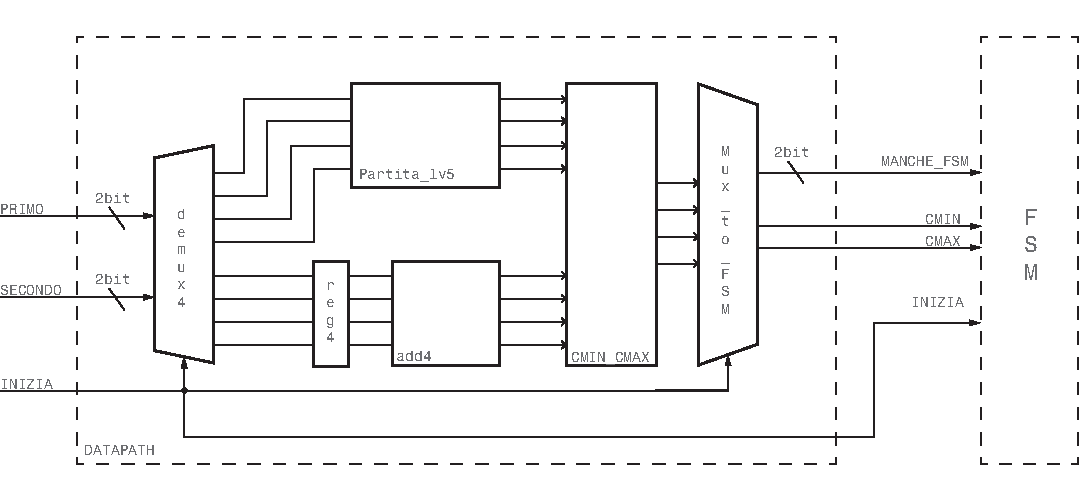
\includegraphics[width=\textwidth]{datapath.pdf}
      \caption{Schema di funzionamento generale del Datapath in SIS}
      \label{img:datapath}
  \end{figure}


\subsection*{Componenti del modello SIS}\label{subsec:component}

La descrizione hardware del sistema è stata sviluppata in SIS utilizzando la descrizione a livello di gate.
Si è scelto di procedere con la descrizione a \textit{gate level} per poter maneggiare la simulazione ad un livello di astrazione piu basso e per poter avere un controllo più preciso sulle risorse utilizzate.
Nello specifico sono stati modellati inizialmente i seguenti componenti:
\vspace*{10pt}

\small
\begin{itemize}
    \item \textbf{Porte Logiche ed elementi base:}
    \begin{itemize}
        \item \textbf{and.blif}: Porta logica AND.
        \item \textbf{not.blif}: Porta logica NOT.
        \item \textbf{notAnd.blif}: Porta logica NAND.
        \item \textbf{nor.blif}: Porta logica NOR.
        \item \textbf{xnor.blif}: Porta logica XNOR.
        \item \textbf{xor.blif}: Porta logica XOR.
        \item \textbf{or.blif}: Porta logica OR.
        \item \textbf{or\_3b.blif}: Porta logica OR a 3 bit.
        \item \textbf{uno.blif}: Costante 1.
        \item \textbf{zero.blif}: Costante 0.
    \end{itemize}
    
    \item \textbf{Operatori Matematici, di Confronto e contatori:}
    \begin{itemize}
        \item \textbf{add4.blif}: Modulo a 5 bit che aggiunge la costante 4.
        \item \textbf{cont5bit.blif}: Contatore a 5 bit.
        \item \textbf{countmanche.blif}: Contatore di manche giocate.
        \item \textbf{maggiore.blif}: Confronto maggiore a 1 bit.
        \item \textbf{maggiore5b.blif}: Confronto maggiore a 5 bit.
        \item \textbf{sum1bit.blif}: Sommatore a 1 bit.
        \item \textbf{sum1bit\_no.blif}: Sommatore a 1 bit (senza riporto).
        \item \textbf{sum2bit.blif}: Sommatore a 2 bit.
    \end{itemize}
    
    \item \textbf{Multiplexer e Demultiplexer:}
    \begin{itemize}
        \item \textbf{Mux.blif}: Multiplexer a 1 bit.
        \item \textbf{Mux\_2b.blif}: Multiplexer a 2 bit.
        \item \textbf{Mux\_5b.blif}: Multiplexer a 5 bit.
        \item \textbf{Mux\_to\_FSM.blif}: Filtro in output dal datapath che reagisce in base al valore di INIZIA.
        \item \textbf{demux1bit.blif}: Demultiplexer a 1 bit.
        \item \textbf{demux4bit.blif}: Demultiplexer a 4 bit.
    \end{itemize}
    
    \item \textbf{Registri:}
    \begin{itemize}
        \item \textbf{Reg.blif}: Registro a 1 bit.
        \item \textbf{Reg\_2b.blif}: Registro a 2 bit.
        \item \textbf{Reg\_4b.blif}: Registro a 4 bit.
        \item \textbf{Reg\_5b.blif}: Registro a 5 bit.
    \end{itemize}
  \end{itemize}

  \normalsize E successivamente implementati in blocchi più complessi:

  \begin{itemize}\small
    \item \textbf{Blocchi Finali e Altri Moduli:}
    \begin{itemize}
        \item \textbf{2b\_to\_3b.blif}: Convertitore delle codifiche di PRIMO e SECONDO in valori a 3 bit per le mosse.
        \item \textbf{CMIN\_CMAX.blif}: Implementazione dei segnali di controllo diretti alla FSM per il conteggio del numero di manche giocate.
        \item \textbf{Check\_Mossa.blif}: Multiplexer modificato per il controllo della mossa del giocatore.
        \item \textbf{Check\_mossa\_2b.blif}: Versione a 2 bit di Check\_Mossa.blif che funziona per due flussi (PRIMO e SECONDO).
        \item \textbf{Gate\_3b.blif}: [da scrivere!].
        \item \textbf{Mossa\_ill.blif}: Implementazione di una mossa ripetuta.
        \item \textbf{tavolino.blif}: Assegna la vittoria in caso di mossa "sconosciuta" all'altro giocatore.
        \item \textbf{Controllo\_Partita.blif}: Modulo che elabora l'annullamento della manche in caso di mossa non permessa.
        \item \textbf{Partita\_lv1.blif}: raggruppamento 1.
        \item \textbf{Partita\_lv2.blif}: raggruppamento 2.
        \item \textbf{Partita\_lv3.blif}: raggruppamento 3.
        \item \textbf{Partita\_lv4.blif}: raggruppamento 4.
        \item \textbf{Partita\_lv5.blif}: raggruppamento 5.
        \item \textbf{DATAPATH.blif}: insieme dei moduli del datapath.
        \item \textbf{FSM.blif}: Macchina a stati finiti.
        \item \textbf{FSMD.blif}: Macchina a stati finiti con datapath.
    \end{itemize}
\end{itemize}

\begin{figure}[h]
  \centering
  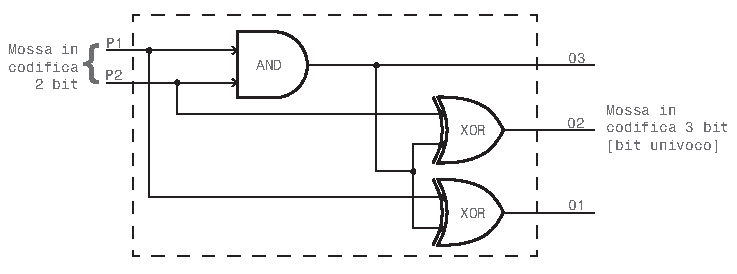
\includegraphics[scale=1]{3bmosse.pdf}
  \caption{Funzionamento del modulo \texttt{2b\_to\_3b.blif}}
  \label{img:3bmosse}
\end{figure}

\begin{figure}[h]
  \centering
  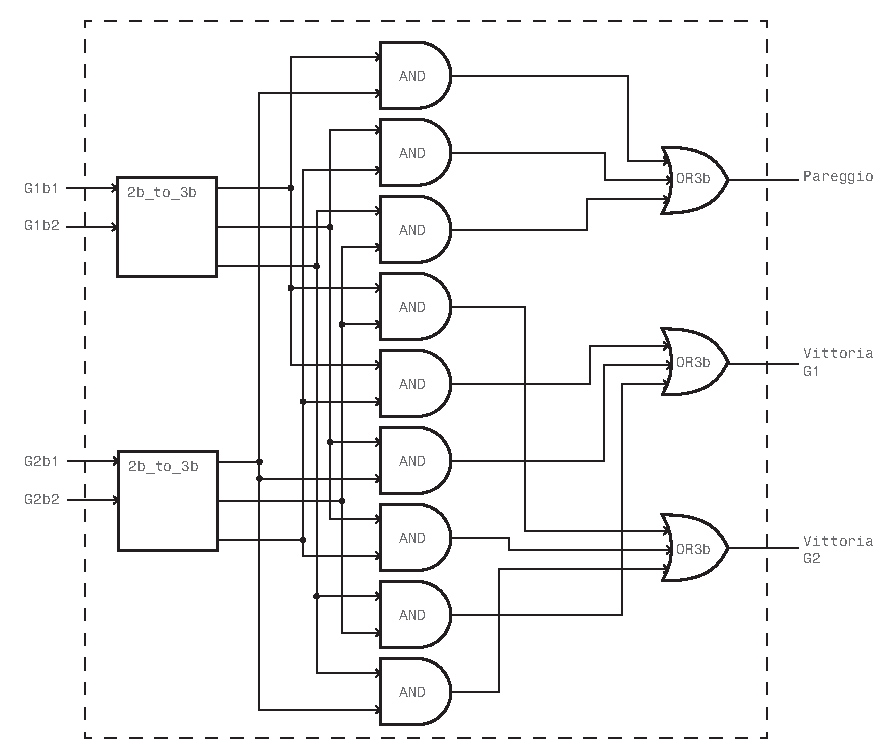
\includegraphics[scale=1]{partitalv1.pdf}
  \caption{Funzionamento del modulo \texttt{Partita\_lv1.blif} }
  \label{img:partitalv1}
\end{figure}

\begin{figure}[h]
  \centering
  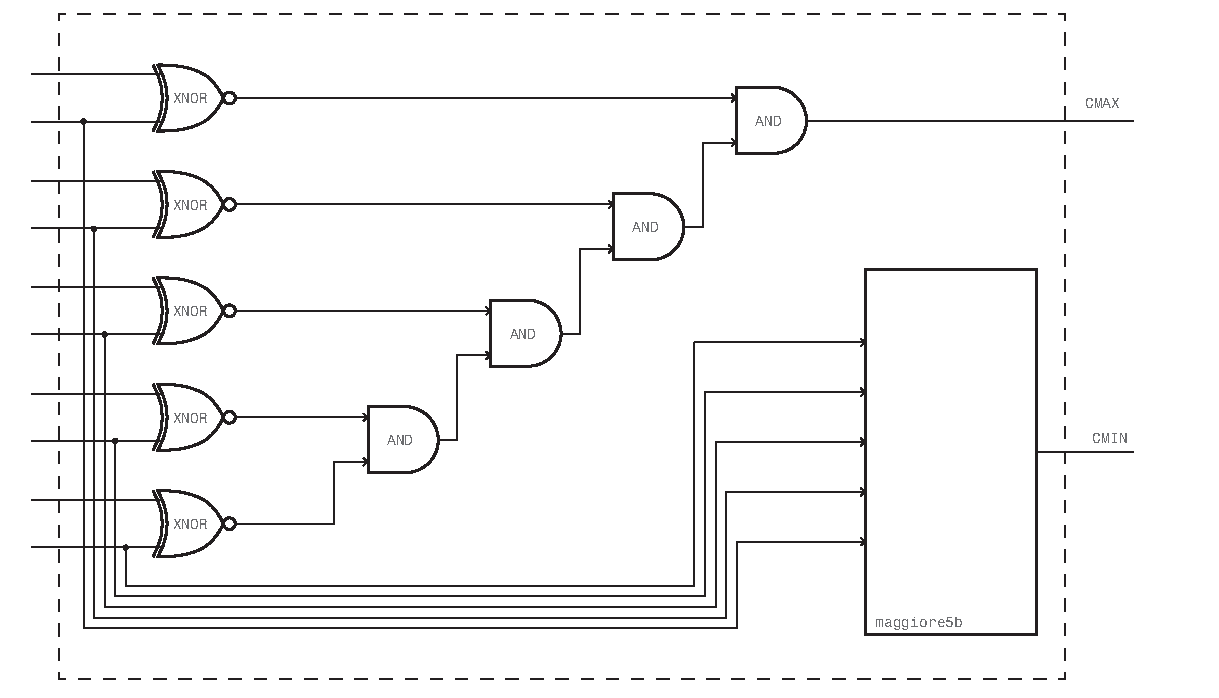
\includegraphics[width=\textwidth]{cmincmax.pdf}
  \caption{Funzionamento del modulo \texttt{CMIN\_CMAX.blif} }
  \label{img:cmincmax}
\end{figure}

\begin{figure}[h]
  \centering
  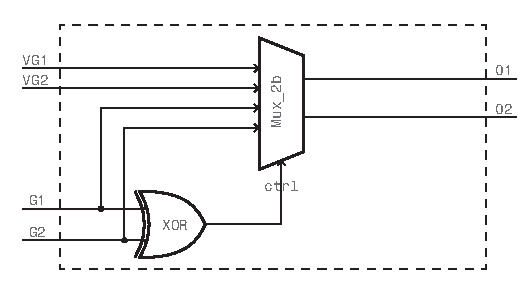
\includegraphics[scale=1]{tavolino.pdf}
  \caption{Funzionamento del modulo \texttt{tavolino.blif} }
  \label{img:tavolino}
\end{figure}


\clearpage % Inserisce tutte le figure prima della pagina successiva


\section{Statistiche del circuito e mapping tecnologico}

Sono stati effettuati due mapping tecnologici del circuito, uno prima dell'ottimizzazione e uno dopo.
L'ottimizzazione ha portato ad una riduzione dei nodi da 474 a 62 e dei letterali (in somma di prodotti) da 969 a 419.

  \begin{figure}[ht]
    \centering
      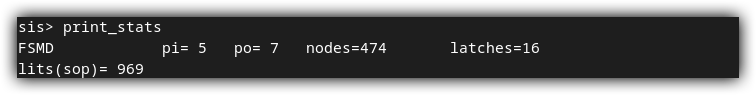
\includegraphics[width=0.86\textwidth]{not_opt.png}
      \caption{statistiche dopo ottimizzazione}
      \label{img:opt.png}
  \end{figure}

  \begin{figure}[h]
    \centering
      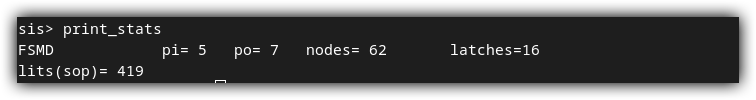
\includegraphics[width=0.86\textwidth]{opt.png}
      \caption{statistiche prima dell'ottimizzazione}
      \label{img:not_opt.png}
  \end{figure}


  Il modello è stato anche mappato sulla libreria tecnologica \texttt{synch.genlib} e sono stati ottenuti i seguenti risultati:
  \begin{figure}[hb]
    \centering
      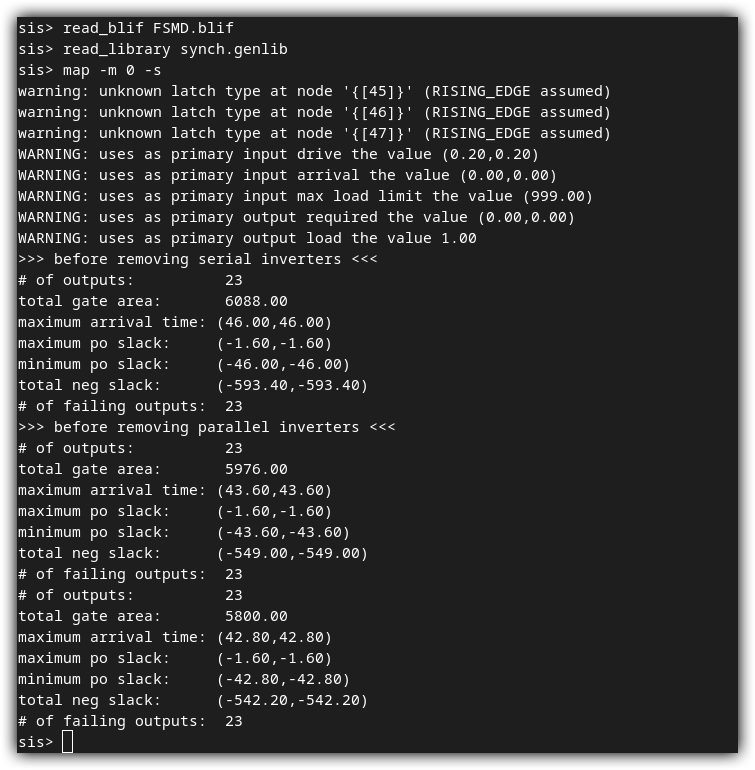
\includegraphics[width=0.86\textwidth]{mapping.png}
      \caption{Statistiche dopo il mapping}
      \label{img:mapping.png}
  \end{figure}





\chapter{Scelte progettuali ed eventuali chiarimenti}
\section{Definizione del comportamento in caso di mossa \textit{"sconosciuta"} al datapath}
Nel caso in cui uno dei giocatori effettui una mossa "nulla" (non riconosciuta come mossa effettiva dalla codifica del datapath, eg. \texttt{PRIMO o SECONDO = 00}) durante una manche, l'altro giocatore vincerà automaticamente.
Tuttavia, è importante notare che questa regola non si applica nel caso in cui un giocatore, proveniente da una manche precedentemente vincente, utilizzi nuovamente la stessa mossa.
In tale situazione, la priorità viene data alla regola presente nelle specifiche che non consente la ripetizione della mossa vincente (per il medesimo giocatore) e rende non valida la manche.

\section{Comportamento del sistema in relazione al segnale \texttt{INIZIA}}
Il segnale \texttt{INIZIA} è stato implementato come un segnale di reset del sistema.
Tuttavia per la sua natura di segnale \textbf{in ingresso} la macchina è stata progettata affinchè al termine di una partita l'elaboratore attenda di ricevere in input il segnale \texttt{INIZIA} per procedere al reset e iniziare una nuova partita.
Al termine di una partia, dopo aver decretato il vincitore (output \texttt{PARTITA} $\neq$ \texttt{00}), dal ciclo di clock successivo il sistema manderà in output \texttt{MANCHE = 00 PARTITA = 00} fintanto che non viene nuovamente attivato lo stato di reset. 

\section{Approfondimento sulla suddivisione delle funzioni tra Datapath e FSM}\label{sec:approfondimento}
La scelta di suddividere le funzioni tra Datapath e FSM è stata guidata da un'analisi delle funzioni chiave che dovrebbe svolgere il sistema, cercando di bilanciare la complessità tra il Datapath e il controllore FSM.
In particolare alcune funzioni, a nostro avviso, combaciavano con la natura combinatoria del Datapath. 

Il confronto delle mosse e la verifica della loro validità, per esempio, coinvolgono principalmente operazioni logiche e confronti diretti tra i dati di input.
Queste operazioni sono più naturalmente implementate in un sistema combinatorio, dove le uscite dipendono solo dagli ingressi attuali senza considerare uno stato interno.\footnote{Si noti che nonostante nel Datapath vengano elaborati direttamente gli input senza tener conto di un eventuale stato del sistema, questo non implica l'assenza di registri funzionali al confronto con dati elaborati in cicli di clock precedenti al calcolo (come per esempio il confronto di una mossa vincente con quella dello stesso giocatore nella manche precedente).}
La progettazione a \textit{gate level} per quanto riguarda la simulazione in SIS, ci ha permesso di gestire il flusso dei dati in maniera puntuale e precisa permettendoci di testare ogni blocco di porte logiche singolarmente per poi unirlo in un sistema più complesso. 

In un sistema a stati finiti sequenziale il focus principale è sulla gestione dello stato attuale del sistema, gli input ricevuti dal Datapath (nel caso dell'elaborato in questione e in generale sul modello di Mealy) e l'elaborazione dello stato prossimo.
Lo spostamento di operazioni logiche complesse dal datapath all'FSM avrebbe reso la logica di controllo inutilmente più complessa, influenzando la chiarezza della progettazione e la manutenibilità del codice.
Nel presente elaborato infatti abbiamo optato per una definizione della FSM ad 8 stati, che ci ha permesso di mantenere un controllo preciso sul flusso di gioco e di gestire in modo chiaro i segnali di output mantenendo una logica combinatoria (all'interno del Datapath) chiara e lineare.


\end{document}
